%%%%%%%%%%%%%%%%%%%%%%%%%%%%%%%%%%%%%%%%%% 10 - 1
\section{Вольт-амперная характеристика лампочки}
\LabHeader{построить и объяснить вольт-амперную характеристику (ВАХ) лампочки.}{Источник постоянного напряжения, реостат, вольтметр, амперметр, лампочка.}
%\begin{wrapfigure}{i}{5.71cm}
%	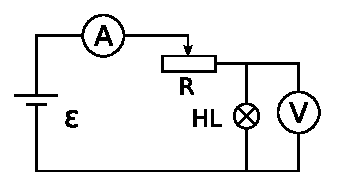
\includegraphics{10kl1-1.pdf}
%    \caption{Схема для снятия ВАХ}
%    \label{fig:10kl-vah:scheme}
%\end{wrapfigure}
\begin{figure}
\end{figure}
\SolveVariant
\begin{figure}[h]
    \centering
    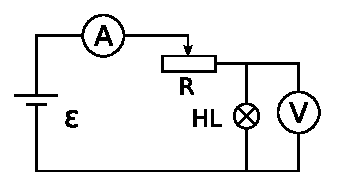
\includegraphics{10kl1-1.pdf}
    \caption{Схема для снятия ВАХ}
    \label{fig:10kl-vah:scheme}
\end{figure}
Соберем схему, изображенную на рис.~\ref{fig:10kl-vah:scheme}. Проведём измерения напряжения и силы тока для 10--20 положений реостата. По полученным данным построим график с прямоугольниками ошибок.
\MesErrors
Для каждой точки на графике существуют только инструментальные погрешности прямых измерений, которые являются табличными значениями для конкретных приборов.
\SchoolBase
\begin{itemize}
    \item Закон Ома. Вольт-амперная характеристика.
    \item Зависимость сопротивления проводника от температуры. 
\end{itemize}
\AdditionalQuestions
\begin{itemize}
    \item Объясните форму вольт-амперной характеристики. {\itshape Наводящий вопрос:} что происходит с сопротивлением лампочки в зависимости от величины тока?\par
    \Answer С ростом тока лампочка нагревается сильнее, температура нити возрастает, и её сопротивление увеличивается. Поэтому график отличается от прямой и с ростом напряжения становится более пологим.
    \item {\itshape(Усложнённый)} Найдите в явном или неявном виде связь между напряжением на лампочке и током через неё, считая, что зависимость мощности теплового излучения от температуры тела имеет вид \(P = \gamma T^4\), а сопротивление проводника подчиняется закону \(R = R_0 + \alpha (T-T_0)\), где \(T\) "--- температура тела, \(T_0\) "--- известная температура, при которой тело имеет известное сопротивление \(R_0\), \(\alpha\) и \(\gamma\) "--- известные коэффициенты. Ответ можно оставить в неявном виде.\par
    \Answer \begin{equation*}
    	\begin{array}{@{}l@{}}
    		P = \gamma T^4 \Rightarrow T=\frac{1}{\gamma^\frac{1}{4}} U^\frac{1}{4} I^\frac{1}{4};\\
    		R = R_0 + \alpha(T-T_0) \Rightarrow U=IR_0+\frac{\alpha}{\gamma^\frac{1}{4}} U^\frac{5}{4} I^\frac{1}{4}-\alpha T_0
    	\end{array}
    \end {equation*}
    Таким образом, зависимость \(I(U)\) получается решением уравнения четвёртой степени относительно~\(I^\frac{1}{4}\).    
\end{itemize}
%%%%%%%%%%%%%%%%%%%%%%%%%%%%%%%%%%%%%%%%%% 10 - 2
\section[Определение ёмкости конденсатора]{Определение электрической ёмкости конденсатора с использованием баллистического гальванометра}
\LabHeader{определить ёмкость неизвестного конденсатора.}{Набор кондансаторов известной ёмкости, конденсатор неизвестной ёмкости, стрелочный микроамперметр в качестве баллистического гальванометра, источник постоянного напряжения, однополюсный переключатель.}
{\itshape Работа предполагает изложение принципов и хода эксперимента лаборантом.}
\SolveVariant
\begin{enumerate}
    \item Соберем схему, изображенную на рис.~\ref{fig:10kl-bg:scheme}. При этом амперметр будет работать по принципу баллистического гальванометра: импульс, приобретаемый стрелкой прибора пропорционален заряду, протекшему через обмотку гальванометра, если время воздействия тока мало по сравнению со временем реакции стрелки, то есть если во время воздействия тока стрелка не успела сместиться на значительный угол.
    \begin{figure}[h]
	    \centering
		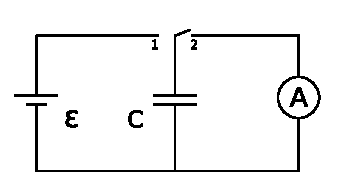
\includegraphics[width=5.71cm]{10kl2-1.pdf}
		\caption{Рабочая схема}
		\label{fig:10kl-bg:scheme}
	\end{figure}
    \item Проградуируем гальванометр. Подключим в качестве конденсатора к схеме конденсатор известной ёмкости. Переключим ключ в положение~1. При этом конденсатор получит заряд \(q= C \varepsilon\), где \(\varepsilon\) "--- ЭДС источника напряжения. Резким движением переведём ключ в положение~2. При этом за короткое время весь заряд конденсатора пройдёт через гальваномер \(A\). Заметим количество делений шкалы~\(N\), на которое отклонилась стрелка. Поскольку напряжение источника "--- постоянное от опыта к опыту, \(N\sim q \Rightarrow N=\alpha C\), где \(\alpha\) "--- постоянный коэффициент.\par
    Для каждого из имеющегося набора конденсаторов известной ёмкости определим \(\alpha_i = \frac{N_i}{C_i}\) и усредним.
    \item Подключив в качестве конденсатора конденсатор неизвестной ёмкости, переведём ключ в положение~1, затем "--- в положение~2. Определим число делений, на которое отклонилась стрелка~\(N_0\). Зная средний коэффициент \(\alpha\), определим ёмкость конденсатора: \(C_0=\alpha N_0\).
\end{enumerate}
Для каждого конденсатора следует повторять опыт несколько раз и брать средний отброс стрелки.
\MesErrors
Поскольку метод подразумевает усреднение {\itshape небольшого} набора результатов (определение \(\alpha\)), учесть это при оценке погрешностей "--- нетривиально. Поэтому будем считать, что \(\alpha\) определена при однократном измерении (такое допущение позволит оценить погрешность сверху). Пусть \(\Delta N\) "--- характерная погрешность определения количества делений, на которое отклоняется стрелка, \(\Delta C\) "--- указанная на конденсаторе погрешность его ёмкости, и \( 1 \) "--- индекс конденсатора с наименьшей ёмкостью из числа известных.
Тогда:
\begin{equation*}
	\varepsilon C_0 = \Delta N \left( \frac{1}{N_1}+\frac{1}{N_0} \right) +\frac{\Delta C}{C_1}
\end{equation*}
\SchoolBase
\begin{itemize}
    \item Электрическая ёмкость. Ёмкость конденсатора.
    \item Баллистический гальванометр.
\end{itemize}
%\AdditionalQuestions
%\begin{itemize}
%    \item вопрос\par
%    \Answer ответ
%\end{itemize}
